Das letzte Szenario ist das einzige, in dem auch außerhalb der Startphase neue Chunks geladen werden. In der Startphase werden alle Chunks in einer Kugel um die Startposition herum geladen. In Szenario 5: Welt-Gehen bewegt sich die Kamera in einer Welt mit Terrain-Generierung konstant in Blickrichtung nach vorne, wie in den Bildschirmfotos in Abbildung~\ref{fig:walk} zu sehen ist. Daher müssen in diesem Szenario schrittweise neue Chunks geladen werden.
\begin{figure}[!htbp]
	\centering
	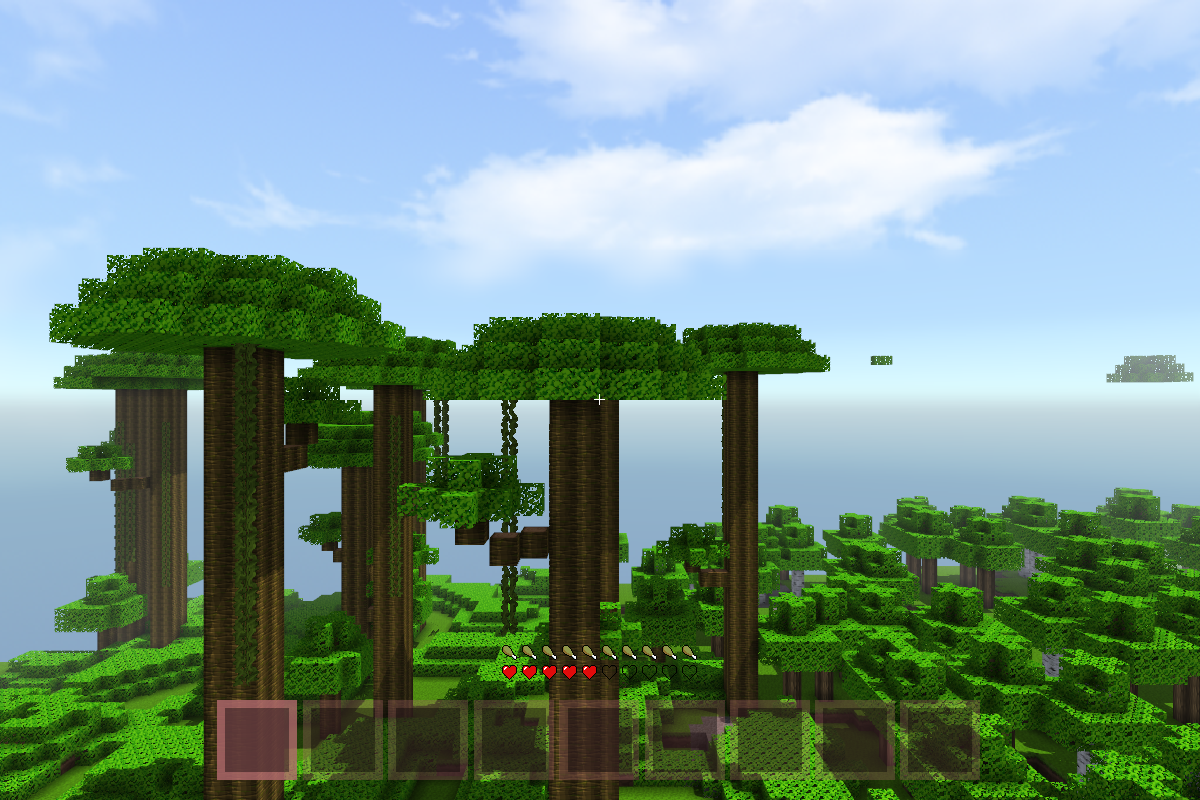
\includegraphics[width=.32\textwidth]{walk-1.png}
	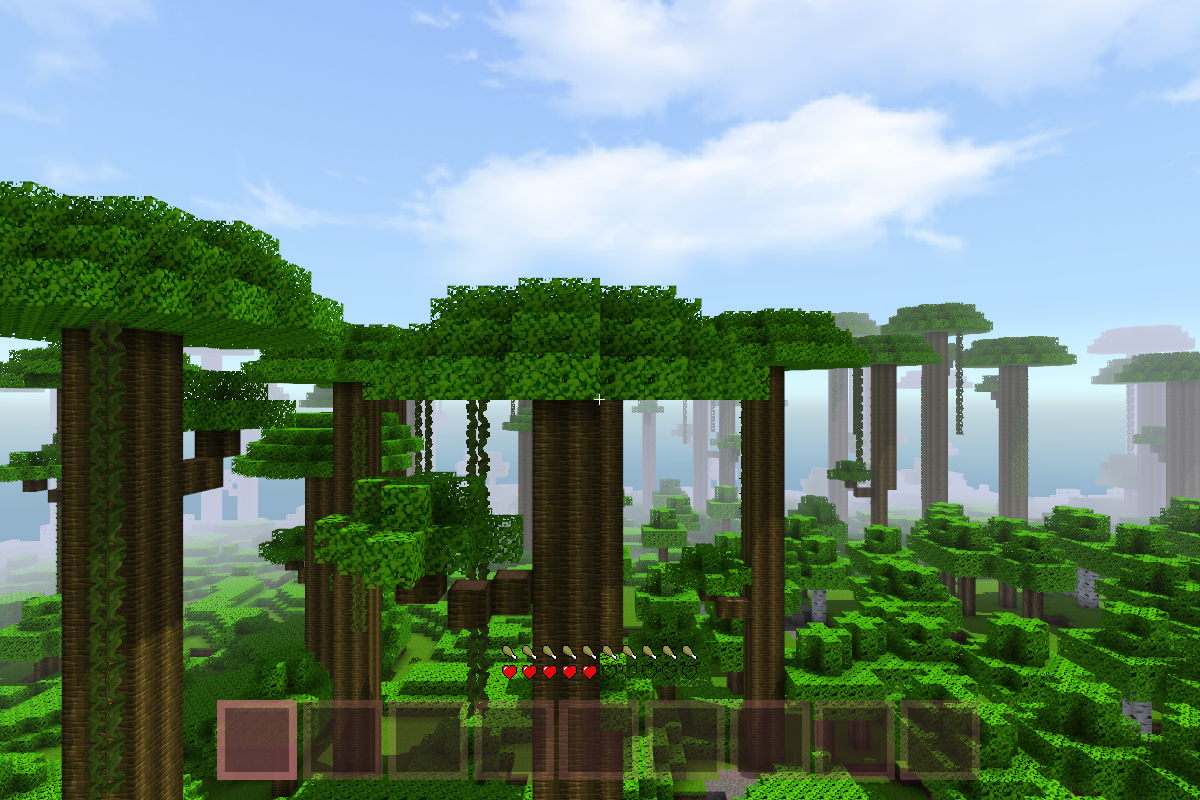
\includegraphics[width=.32\textwidth]{walk-2.png}
	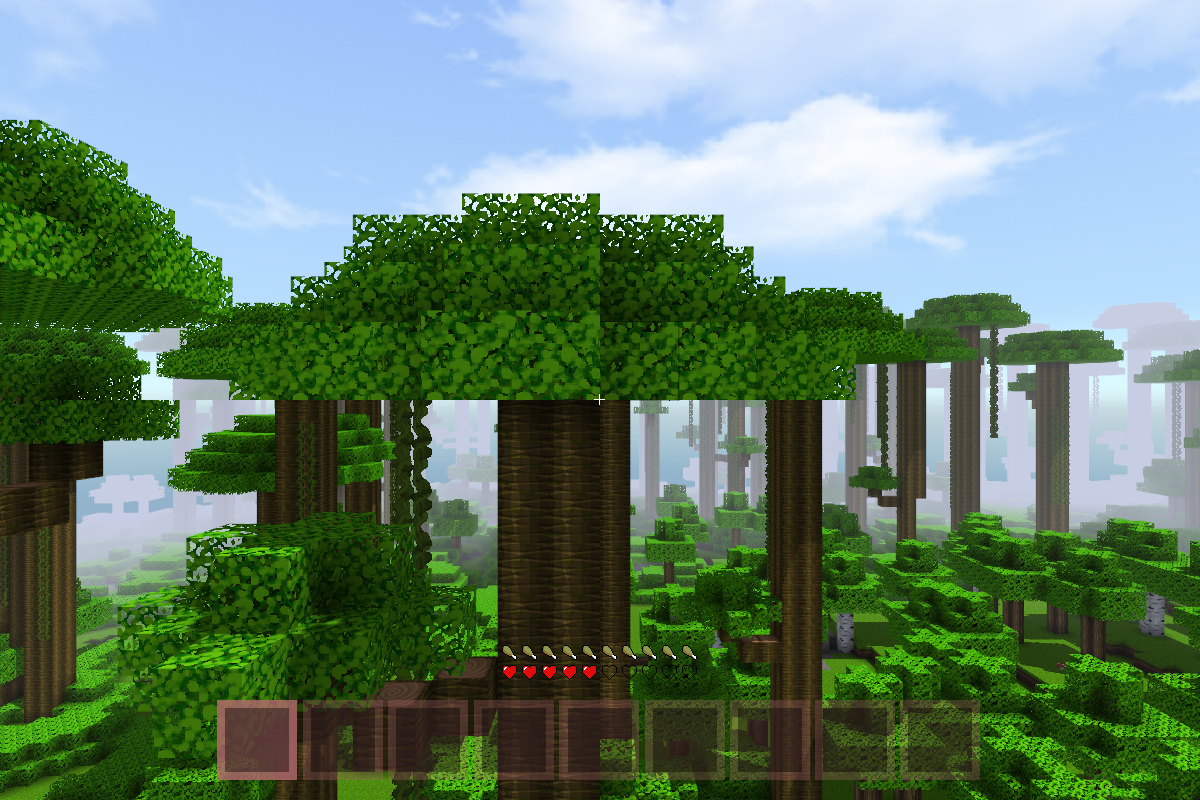
\includegraphics[width=.32\textwidth]{walk-3.png}
	\caption[Reihe von Bildschirmfotos, die die Fortbewegung in Szenario 5 zeigt.]{Reihe von Bildschirmfotos, die die Fortbewegung in Szenario 5 zeigt. Die Bildschirmfotos haben einen Zeitabstand von \SI{1000}{\milli\second}. Im Hintergrund sind die neu geladenen Chunks zu erkennen.}\label{fig:walk}
\end{figure}

Für die folgenden Messungen wird weiterhin der Seed 0 genutzt. Für dieses Szenario existieren außerdem Messungen für die Seeds 3 und 10. Die Graphen dieser Messungen sind zusammen mit den Graphen der anderen Messungen gesammelt in Anhang~\vref{appendix:plots} zu sehen. Die Daten werden in Abschnitt~\ref{sec:zusammenfassung} mit den restlichen Daten zusammenfassend verglichen.

\paragraph{\ac{fps}}
Der Verlauf der Bildwiederholrate in Szenario 5 wird von Abbildung~\ref{fig:seed-0-walk-fps} dargestellt. Wie in allen bisherigen Szenarien ist auch in Szenario Welt-Gehen eine Verzögerung des Starts von \sysB{} im Vergleich zu \sysA{} zu erkennen.
\begin{figure}[!htbp]
	\fpsplot{seed-0-walk}
	\caption{Graph des Verlaufs der Framerate in Szenario 5: Welt-Gehen mit Seed 0.}\label{fig:seed-0-walk-fps}
\end{figure}
Der Verlauf der Framerate ist in beiden Systemen deutlich unruhiger als in allen bisherigen Szenarien. \sysA{} erreicht im Durchschnitt \SI{128}{\fps}. In \sysB{} steigt die Bildwiederholrate um \SI{198}{\percent} auf durchschnittlich \SI{381}{\fps}. Während die Bildwiederholrate in \sysA{} unter Vernachlässigung des unruhigen Verhaltens in etwa konstant bleibt, steigt sie in \sysB{} aus einem unbekannten Grund kontinuierlich langsam an. So wird zu Beginn bei Sekunde 23 eine maximale Framerate von \SI{354}{\fps} gemessen. Diese steigt bis zum Ende der Messung bis zu \SI{515}{\fps} bei Sekunde 58. Dieser Anstieg scheint allerdings nicht in der Beschaffenheit des Szenarios begründet zu sein, da dieses Verhalten in den Messungen desselben Szenarios mit den Seeds 3 und 10 (siehe Anhang~\vref{appendix:fpsplots}) nicht zu sehen ist. 

\paragraph{\ac{cpu}}
Wie der Verlauf der Bildwiederholrate ist auch die Auslastung der \ac{cpu} deutlich unsteter als in den bisherigen Szenarien, in denen sie in der Hauptphase beinahe konstant ist. In Abbildung~\ref{fig:seed-0-walk-cpu} ist der Graph des Auslastungs-Verlaufs zu sehen.
\begin{figure}[!htbp]
	\cpuplot{seed-0-walk}
	\caption[Graph des Verlaufs der \glsentryshort{cpu}-Auslastung in Szenario 5: Welt-Gehen mit Seed 0.]{Graph des Verlaufs der \ac{cpu}-Auslastung in Szenario 5: Welt-Gehen mit Seed 0.}\label{fig:seed-0-walk-cpu}
\end{figure}
Im Gegensatz zu Szenario 4: Welt-Rotation, scheint die Messung in diesem Szenario in beiden Systemen zwar gleichzeitig zu sein, dennoch ist der Trend der vorherigen Messungen zu einer längeren \ac{cpu}-Auslastung durch \sysB{} in der Anfangsphase auch hier nicht zu erkennen. Die Messungen mit anderen Seeds, die in Anhang~\vref{appendix:cpuplots} mit dargestellt sind, bestätigen diesen Befund.

Im Gegensatz zu den anderen Szenarien steigt in diesem Szenario die Auslastung der \ac{cpu} auch während der Hauptphase in beiden Systemen immer wieder merklich an. \sysA{} hat eine durchschnittliche Auslastung von \SI{27}{\percent} und \sysB{} zeigt eine Durchschnittsauslastung von \SI{36}{\percent}. Dieser Anstieg ist auf die während der Hauptphase zu ladenden Chunks zurückzuführen. Hierfür werden in beiden Systemen alle Hardware-Threads genutzt, wie in den vorherigen Kapiteln beschrieben worden ist. Damit erhöht sich auch die Gesamtauslastung der \ac{cpu}. Dass in dem Graphen in der Hauptphase keine Auslastungsspitzen nahe \SI{100}{\percent} zu sehen sind, liegt vermutlich an einer zu geringen zeitlichen Auflösung der Messung.

\paragraph{\ac{gpu}}
Auch die \ac{gpu} erfährt in diesem Szenario eine variable Auslastung. Die Ausschläge sind, wie Abbildung~\ref{fig:seed-0-walk-gpu} zeigt, kleiner als in Szenario Welt-Rotation jedoch deutlich häufiger und unregelmäßiger.
\begin{figure}[!htbp]
	\gpuplot{seed-0-walk}
	\caption[Graph des Verlaufs der \glsentryshort{gpu}-Auslastung in Szenario 5: Welt-Gehen mit Seed 0.]{Graph des Verlaufs der \ac{gpu}-Auslastung in Szenario 5: Welt-Gehen mit Seed 0.}\label{fig:seed-0-walk-gpu}
\end{figure}
In \sysA{} lässt sich eine durchschnittliche Auslastung von \SI{34}{\percent} messen, \sysB{} zeigt \SI{42}{\percent} \ac{gpu}-Auslastung und damit eine Steigerung von \SI{24}{\percent}.

Auffällig ist, dass entgegen des Verhaltens der Bildwiederholrate die Auslastung der \ac{gpu} in \sysB{} während der Messung tendenziell sinkt. Dieses Verhalten lässt sich in den Messungen mit weiteren Seeds nicht reproduzieren (siehe Anhänge~\vref{appendix:fpsplots} und \vref{appendix:gpuplots}). Dort sind sowohl Framerate als auch \ac{gpu}-Auslastung, ausgenommen der Schwankungen, gleichbleibend. Es bleibt zu überprüfen, ob sich die Messergebnisse des Szenarios bei Verwendung desselben Seeds $0$ wiederholen oder nicht.

\paragraph{\ac{ram}}
Abschließend wird nun noch der in Abbildung~\ref{fig:seed-0-walk-mem} dargestellte Speicherverbrauch betrachtet. In beiden Systemen steigt der Tenured-Speicherverbrauch an, während der Gesamtverbrauch über die gemessene Zeit in der Hauptphase konstant ist.
\begin{figure}[!htbp]
	\memplot[xticklabels={,,},xlabel={}]{seed-0-walk-multi-mem.csv}{\sysA{}}
	\\\memplot{seed-0-walk-multi-mem.csv}{\sysB{}}
	\caption{Graph des Verlaufs der Speichernutzung in Szenario 5: Welt-Gehen mit Seed 0.}\label{fig:seed-0-walk-mem}
\end{figure} 
\sysA{} besitzt einen Speicherverbrauch von \SI{1215}{\mega\byte} .\sysB{} nutzt mit \SI{1881}{\mega\byte} durchschnittlich \SI{55}{\percent} mehr \ac{ram}. Der kurzfristige Speicherverbrauch liegt bei \SI{114}{\mega\byte\per\second} in \sysA{}. Das ist das Maximum des Systems über alle Szenarien hinweg. In \sysB{} wird ein Speicherbedarf von \SI{248}{\mega\byte\per\second} für die Erzeugung kurzfristig genutzter Objekte gemessen. Damit ergibt sich in diesem Szenario ein Anstieg von \SI{118}{\percent}. 

Besonders interessant ist in diesem Szenario der Speicherverbrauch der langlebigen Objekte~(Tenured). In allen anderen Szenarien ist diese Menge über den Großteil der Messung konstant.
In Szenario 5: Welt-Gehen steigt dieser zum ersten Mal während der Hauptphase stetig. In \sysA{} wird ein Anstieg von \SI{401}{\mega\byte} in Sekunde 25 zu \SI{705}{\mega\byte} in Sekunde 54 gemessen. In \sysB{} steigt die Nutzung von \SI{585}{\mega\byte} auf \SI{800}{\mega\byte}. Das ist ein dauerhafter Anstieg von \SI{10}{\mega\byte\per\second} in \sysA{} und ein Anstieg von \SI{7}{\mega\byte\per\second} in \sysB{}. Diese Tatsache liefert ein Indiz für die Existenz von Speicherlecks in der Blocklib. Um diesen Anschein zu bestätigen oder zu entkräften, wäre es sinnvoll in der Zukunft auch längere Messungen durchzuführen. Eine mögliche Erklärung für den steten Anstieg könnte auch sein, dass in der Messung während der Hauptphase keine Garbage-Collection stattfindet und so nur scheinbar ein stetig steigender Speicherbedarf entsteht.

